%!TEX root = ../thesis.tex
%*******************************************************************************
%****************************** Fourth Chapter **********************************
%*******************************************************************************
\chapter{Results}

% **************************** Define Graphics Path **************************

\graphicspath{{Chapter4/Figs/Vector/}{Chapter4/Figs/}}

\section{Non-Parametric}
Non-parametric equations have the benefit of not requiring the minimisation function. Due to this, all testing of these algorithms were undertaken on a standard laptop. These also tend to be the easiest to implement, as uncovered in Chapter~\ref{ch:method}. Particularly important is the Monte Carlo method as this allows shows what should be a minimum baseline to achieve.

\subsection{Monte Carlo}
The first non-parametised algorithm discussed in Chapter~\ref{ch:method} was the Monte Carlo method. Due to the non-parametric nature of this algorithm, execution was simply carried out on the test data set. Results are presented in Figure~\ref{fig:MCTestSet}, demonstrating a final weighted mse of ${0.184\pm{}0.018}$.
\begin{figure}[H]
    \begin{center}
        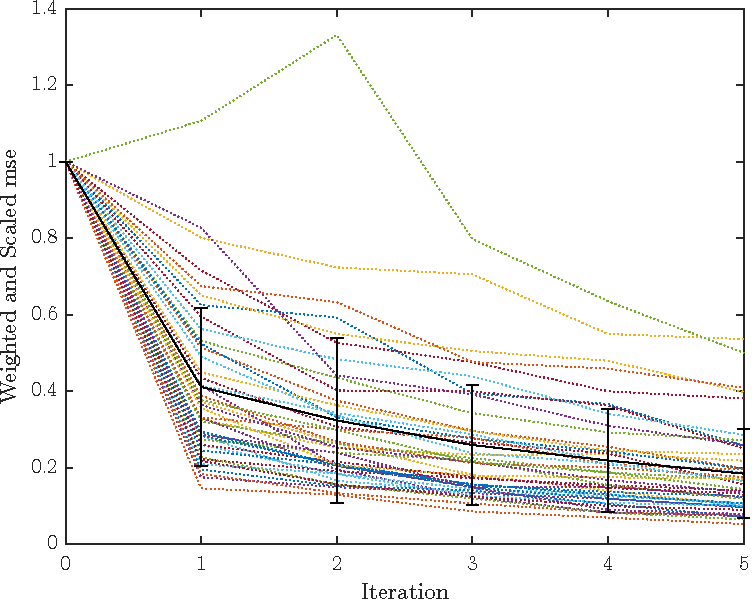
\includegraphics{dumb1.pdf}
        \caption[Monte Carlo]{Results of Monte Carlo sampling on the test datasets. Dotted lines represent the individual scoring for the data sets and the solid line shows the mean results at each iteration with error bars of $\frac{\sigma{}}{\sqrt{n-1}}$.}
        \label{fig:MCTestSet}
    \end{center}
\end{figure}

\subsection{Greedy}
Likewise, the greedy algorithm was tested, with results presented in Figure~\ref{fig:GreedyTestSet}. Here, a final weighted mse of ${0.323\pm{}0.039}$ was found indicating a worse scoring despite more precise results when compared to Monte Carlo - the base case.
\begin{figure}[h]
    \begin{center}
        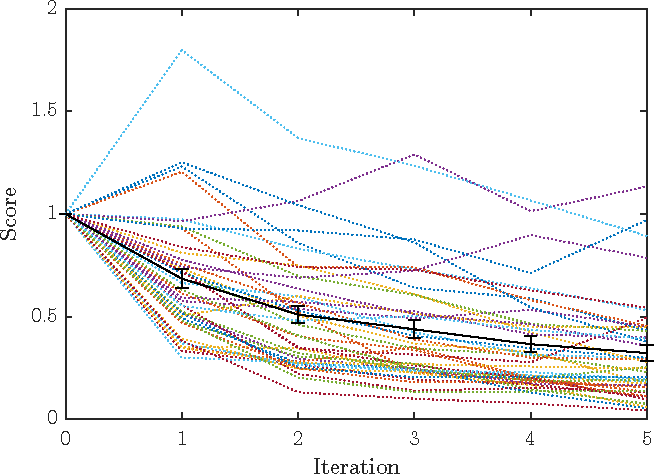
\includegraphics{greedy1.pdf}
        \caption[Greedy]{Results of greedy sampling on the test datasets. Dotted lines represent the individual scoring for the data sets and the solid line shows the mean results at each iteration with error bars of 1 standard deviation.}
        \label{fig:GreedyTestSet}
    \end{center}
\end{figure}

\subsection{ROD Sampling}
The final non-parametic algorithm to be tested was ROD. A final weighted mse of ${0.211\pm{}0.022}$, over performing the previous two algorithms in both accuracy and precision.

\begin{figure}[H]
    \begin{center}
        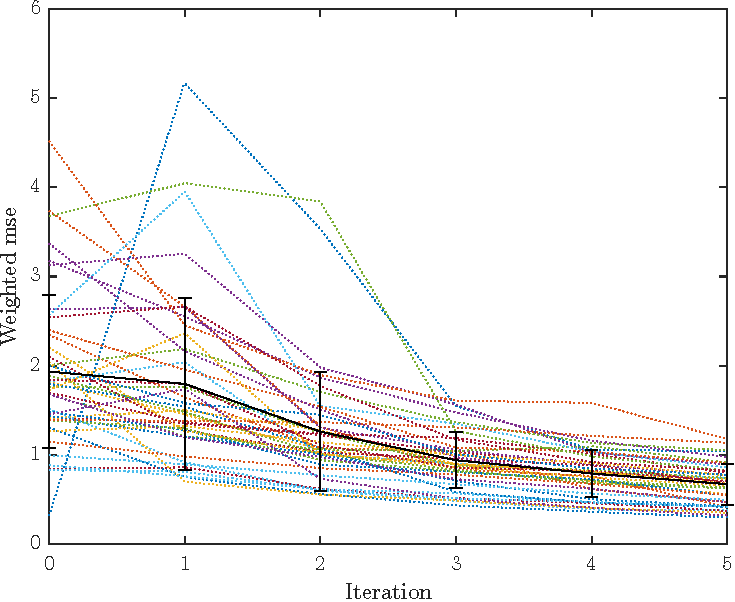
\includegraphics{rod1.pdf}
        \caption[ROD]{Results of ROD sampling on the test datasets. Dotted lines represent the individual scoring for the data sets and the solid line shows the mean results at each iteration with error bars of 1 standard deviation.}
        \label{fig:RODTestSet}
    \end{center}
\end{figure}

\section{Parametric}
Parametric algorithms require a minimisation procedure on the training set. This leads to a computationally challenging script, and for this the author is grateful for the services provided by the HPC \cite{HPC}.
\subsection{Hotspot Clusters}

${0.155\pm{}0.020}$
${0.145\pm{}0.009}$
${0.143\pm{}0.016}$

\begin{figure}[H]
    \begin{center}
        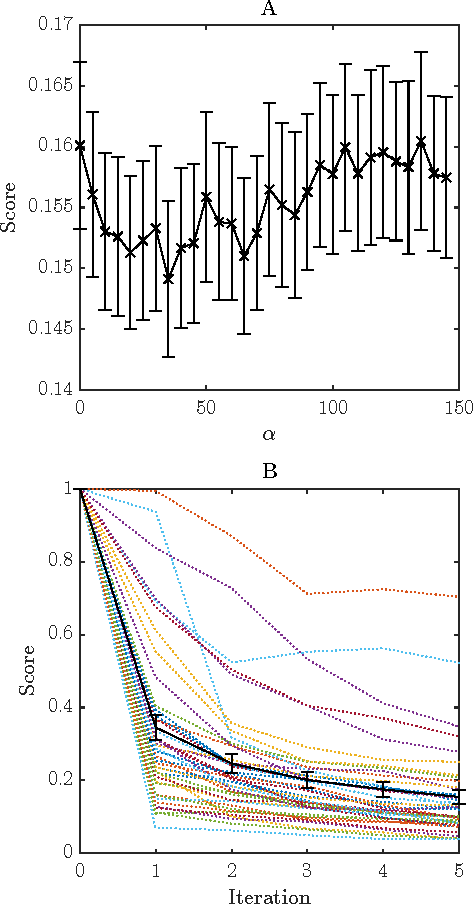
\includegraphics{cluster.pdf}
    \end{center}
\end{figure}
\begin{figure}[H]
    \begin{center}
        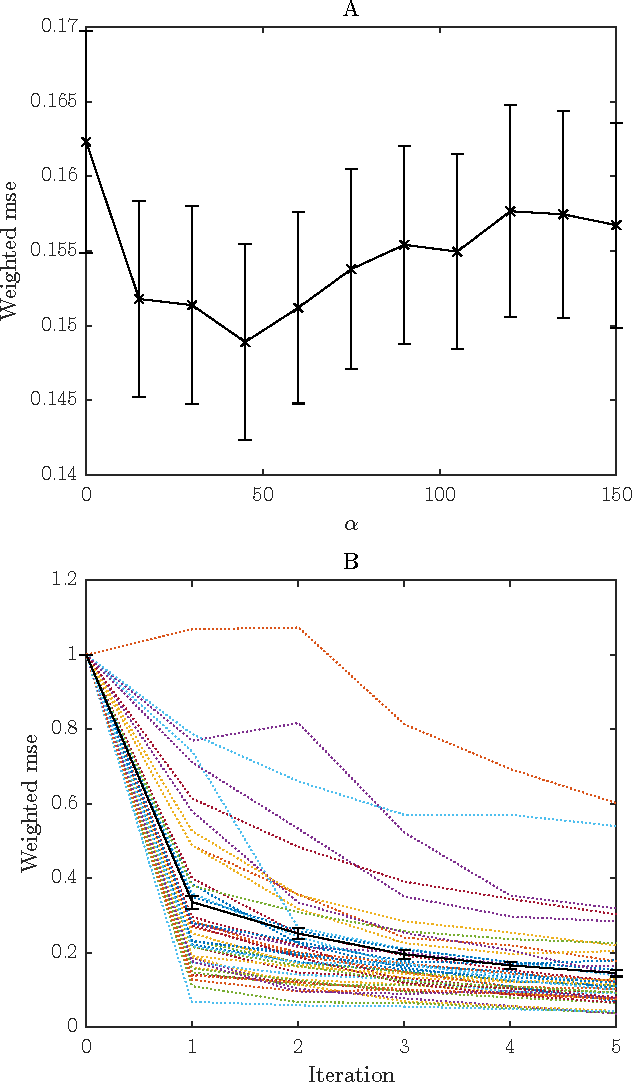
\includegraphics{clusterII.pdf}
    \end{center}
\end{figure}
\begin{figure}[H]
    \begin{center}
        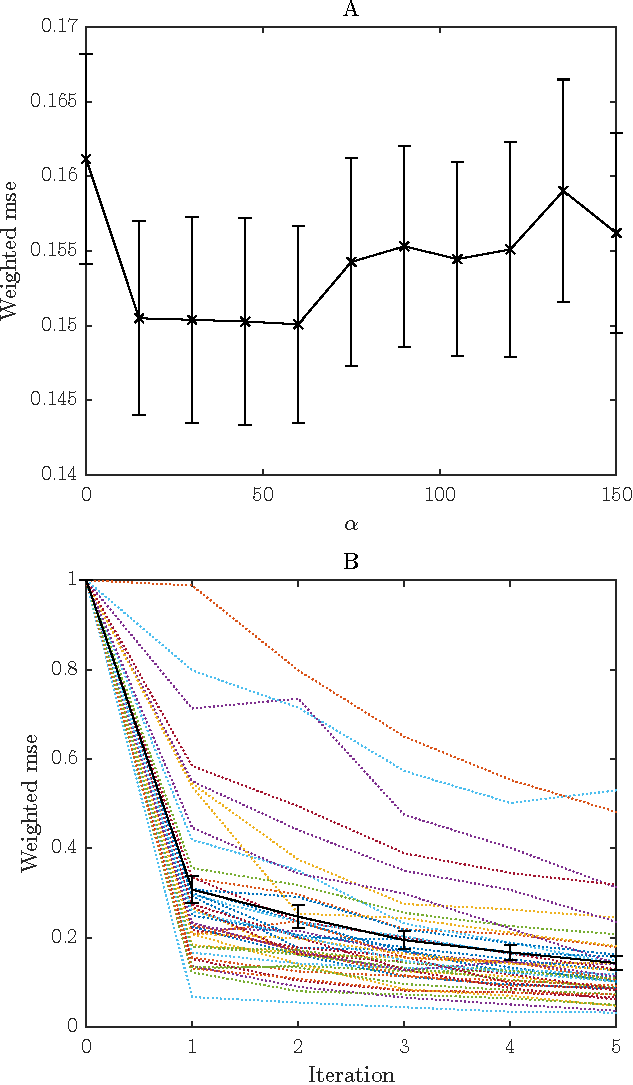
\includegraphics{clusterIII.pdf}
    \end{center}
\end{figure}
\subsection{ROD with Greed}
When testing the ROD with greed sampling method, it was found that despite the weighting towards higher value targets, no improvement was seen over ROD with $\alpha{}=0.06$, with $\alpha$ defined in \ref{eq:rodAndGreed}. However, the tolerance at small $\alpha$ is low, as shown with the errors attached during parameter fitting. This gives a score of ${0.206\pm{}0.011}$, a slight improvement over simply using ROD.

\begin{figure}[H]
    \begin{center}
        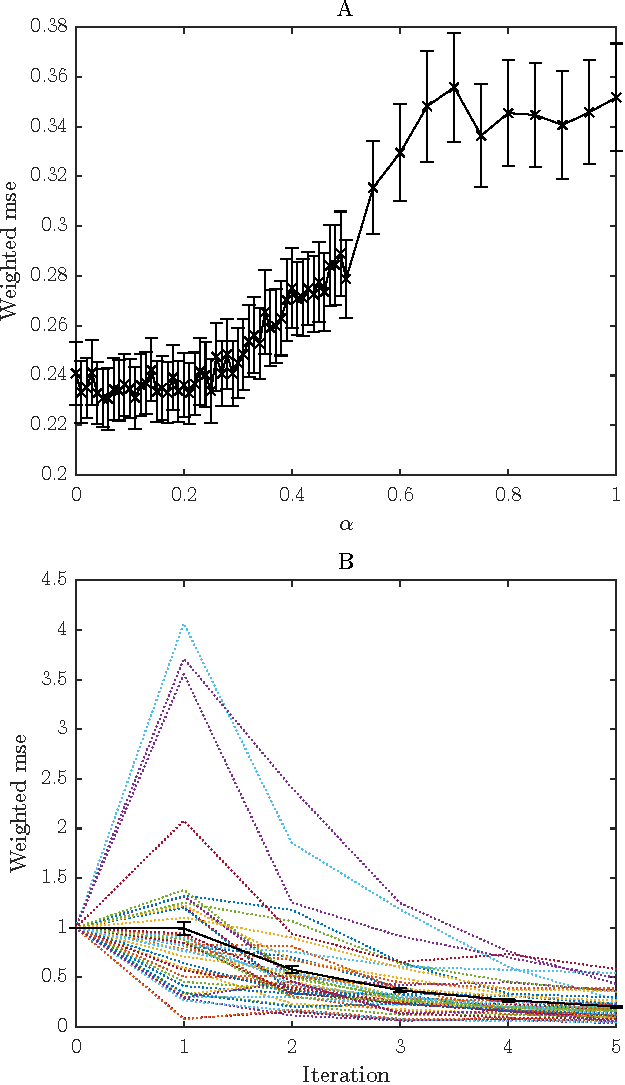
\includegraphics{rodGreedParam.pdf}
    \end{center}
\end{figure}

% \section{Special Case: COVID-19}